% För digital användning
\pdfminorversion=7
\documentclass[12pt,a4paper,notitlepage,twoside]{article}

\makeatletter
\def\app@exe{\immediate\write18}
\def\precompile{%
\IfFileExists{./output.log}{ % Utför endast om ShareLaTeX
  \IfFileExists{./sjungboken2.idx}{}% Kör inte make.sh igen när pdflatex kallas i make
    {
        \app@exe{chmod +x make.sh}%
        \app@exe{./make.sh}%
    }
  }
 }{}
\makeatother

\precompile

\usepackage[utf8]{inputenc}
\usepackage{formatmall}
\usepackage[swedish]{babel}
\usepackage{textfit}
\usepackage{fancyhdr}
\usepackage[hang,small,bf]{caption}
\usepackage{graphicx}
\usepackage{longtable}
\usepackage{makeidx}
\usepackage{multicol}
\usepackage{hyperref}
\usepackage{pdfpages}

% Newpages - enable for book, disable for sanghafte
\newcommand{\newp}{\newpage}

% Include songs
\newcommand{\inputsong}[1]{\input{texter/#1.tex}}

\fancyhead[L]{\large Encyclopedia Gasquica}
\fancyhead[R]{\large F-sektionens sjungbok}
\fancyfoot[C]{}
\renewcommand{\footrulewidth}{0.5pt}
\pagestyle{fancy}
\makeindex
%\paperwidth = 10.45 cm
%\paperheight = 14.85 cm
%\voffset = 0.41 cm %vertikal offset
%\hoffset = -2 cm
%\topmargin = 0 cm %marginal ovanför header
\headheight = 1 cm %headerhöjd
%\headsep = 0 cm %mellan header och body
%\textheight = 13 cm %bodyns höjd
%\textwidth = 9 cm
%\oddsidemargin = 0 cm %marginalen på udda sidor


\begin{document}

\begin{flushleft}
{\Huge Förord\\}
\end{flushleft}

{\large
\setlength{\parskip}{0.8em}
I handen har du nu Encyclopedia Gasquica, den sjungbok som finns för medlemmar av Fysikteknologsektionen.
Boken är en del i den långa tradition som funnits på Chalmers av att anordna sittningar.

Även om sittningarna i tidernas begynnelse såg annorlunda ut, så har de mycket gemensamt med idag.
En god måltid inmundigas, det sjungs och det dricks.
Kom dock ihåg att god sed kännetecknas av att inte dricka utan att sjunga.
Ty, kan man inte sjunga längre är det en god indikation på att man skall minska intagandet av dryck.

Jag som i mitt anletes svett har editerat detta magnifika verk, heter Thomas.
Sjungboken hade dock aldrig funnits utan alla \\tidigare sångförmän, diktare, låtskrivare, musiker, Bellman, Jonas Ahlströmer, Chalmersspexet, Barocken,
Dennis, Elmer, Preisz, Kvickan, Roine, Ewok, An'li, Anders Eldeman, Olofponken, CING, många fler eller en god whisky.
Jag och alla som har hjälpt mig vill värna om en sångskatt som decennier av fysikteknologer har förädlat.
Vem kan glömma gamla fysikaliska klassiker som ''Man ska ha MATLAB'', ''Min punsch'' eller ''Bara kvant''?

Det är med stolthet och framtidstro som jag till sist vill önska dig stor glädje vid nyttjandet av sjungboken.

\vspace{0.5cm}
\begin{flushright}
\textbf{Thomas Lovén}\\
Sångförman 2007-2010
\end{flushright}
}

\newpage

{\large
\setlength{\parskip}{0.8em}
\textit{Med nya tider kommer nya teknologier.}\\
\textit{Med nya teknologier kommer nya möjligheter.}

Min resa i sångernas värld började år 2014 när jag blev Nollan på Teknisk fysik. Jag insåg efter en rad sittningar att sånghäftena inte var särskilt tilltalande. Det visade sig också att det inte heller fanns ett snabbt, enkelt och standardiserat sätt att skapa dem.
Därför började jag under F6-aspning 2015 att utveckla en mall för sånghäften i LaTeX i hopp om att kunna använda den under mitt år som sexmästerist.
Det blev en stor succé och medlemmar från alla sektionens hörn ville använda min mall.

Jag insåg att det fanns mer att göra och bestämde mig därför att bli sångförman i LP3 2016.
Jag hade visioner om ett sånghäfte och en sjungbok som levde i symbios (gemensam sångdatabas).
Först lade jag upp den dåvarande sjungboken på ftek.se, vilket var uppskattat eftersom den inte delades ut till Nollan från och med 2016.
Jag lade också upp en guide för mallen på ftek.se så att den inte skulle falla i glömska.
Men det tog mig ett år att samla modet för att uppnå min vision, då jag i början av sommaren 2017 skapade GitHub repos för mallen och boken.
Efter dagars kodande, debuggande och frenetiskt letande på StackExchange var det klart.

Jag har därmed, via sångförmännen, grott det första fröet för en ljuvstämmig framtid; en framtid där \textbf{alla} sektionens medlemmar kan förvalta och bevara sektionens sångtraditioner tillsammans. Och jag hoppas att du vill vara med på resan...

\begin{flushright}
\textbf{Johan ''Wello'' Winther}\\
Sångförman 2016-2018\\
PR-chef i F6 15/16\\
Vice ordförande i SNF 16/17\\
Informationsansvarig i F-styret 17/18\\
\end{flushright}
}

\newpage
\begin{flushleft}
{\Huge Supregler anno 1900\\}
\end{flushleft}
{\large
Den ganska märklliga svenska supseden är en fullkomlig nationell egenart, som inte tillämpas utomlands.
Dess historia kan spåras till urtiden, varifrån den konserverats inom kloster och sedemera fortlevat inom skråaväsendet.
Vikingarna saknade överflöd på dryckeskärl, varför ett och samma horn ofta gick från man till man runt bänklaget.
Först drack hövdingen.
Därmed blev drickandet fritt i det att övriga deltagare i kalaset fingo tillfälle att begagna kärlet.
När detta gått laget runt och återkommmit till hövdingen var drickandet slut.
Tal hålels inte till brännvin.
Orsaken särtill kan sökas i det svenska brännvinsglasets konstruktion.
Detta föreställer en tratt och var även till sitt ursprung en sådan.
För att hålla drycken kvar, måste man täppa pipen med ett finger.
På det sättet kunde man inte i oändlihet hålla brännvinet i beredskap
utan tvingades att hastigt svälja supen i ett svep för att få fingret och handen fria.
Med utgångspunkt från dessa traditionella förhållanden
är det lättare att förstå de numera gällande lagarna för svenskt skålande.
\begin{enumerate}
\item En skål är ett tyst tal för den som tilldrickas.
\item En skål får ej föreslås innan det första talet hållits.
\item Det åligger värden att dricka med varje gäst.
\item Den som fått emottaga en skål är skyldig att besvara den.
\item Personer av lägre rang bör ej dricka med person av högre rang,
innan denne druckit med den lägre placerad.*
\end{enumerate}
\newpage

* Rangrulla:
\begin{itemize}
    \item Egen operaloge ger: 6 poäng.
    \item Eget stenhus i staden ger: 5 poäng.
    \item Eget hus på landet ger: 4 poäng.
    \item Varje miljon kronor på banken ger: 2 poäng.
    \item Egen landå med fyrspann ger: 1 poäng.
    \item En vinkällare ger: 1 poäng.
    \item En känd anhörig ger $\frac{1}{2}$ poäng.
    \item God allmänbildning ger $\frac{1}{8}$ poäng.
\end{itemize}
}

\begin{flushleft}
{\Huge Avtackning\\}
\end{flushleft}
{\large
Som tack för ett framträdande sjunges följande:

\begin{flushleft}
Det där det gjorde de fan så bra!\\
En skål uti botten för NN vi ta\\
\repopen Hugg i och dra, hej! \repclose\\
En skål uti botten för NN vi ta\\
Och alla så dricka vi nu NN till\\
Och NN säger\\
(Solo NN)\\
För det var i vår ungdoms fagraste vår\\
Vi drack varandra till och vi sade gutår!\\
\end{flushleft}
}


\setcounter{section}{6}
\fancyfoot[RO,LE]{\large Sektionssången}
\begin{flushleft}
\section{Sektionssången}
\end{flushleft}

\setcounter{song}{-1}
\inputsong{dragosdragos}


\setcounter{section}{1}
\fancyfoot[RO,LE]{\large Folksånger}
\inputsong{dugamla}

\newpage

\inputsong{vielsker}

\newpage

\inputsong{vartland}

\inputsong{yndigtland}

\newpage

\inputsong{kungssangen}

\newpage

\inputsong{varmeland}

\newpage

\inputsong{livet}

\newpage

\inputsong{studentsangen}

\inputsong{rektorssangen}


\stepcounter{section}
\fancyfoot[RO,LE]{\large Snapsvisor}
\begin{flushleft}
\section{Snapsvisor}
{\Large
I vårt avlånga land står många olika sorters snaps att finna, vissa godare
än andra. Självklart väljer var person snaps efter eget tycke, men en snaps som innehar en viss särställning gentemot andra är
Bäska droppar. Trots sin något avancerade smak har den blivit så populär att den länge varit ett givet inslag på de flesta Chalmersfester. Viss varsamhet bör
dock iakttagas vid intagande av snapsen, då det är lätt att bli styv i korken efter ett alltför ymnigt pokulerande.
}
\end{flushleft}

\vspace{2cm}
\begin{center}

\includegraphics[width=6cm]{bilder/snaps.eps}
\end{center}

\newpage
\inputsong{helan}
\inputsong{hellandgore}
\newpage
%\inputsong{erland}
\inputsong{thtyrkethaft}
\inputsong{jamadendrickas}
\newpage
\inputsong{halvan}
\inputsong{merabrannvin}
\newpage
\inputsong{masen}
\newpage
\inputsong{manen}
\inputsong{moosen}
\newpage
\inputsong{mesen}
\inputsong{musen}
\newpage
\inputsong{porthos}
\newpage
\inputsong{snusen}
%Bortkommenterad 2014
%\newpage
%\inputsong{handelsvisan}
\newpage
\inputsong{lyftet}
\newpage
\inputsong{rattata}
\inputsong{nutarviden}
\newpage
\inputsong{tjutrean}
\inputsong{opriver}
\inputsong{byssanlull}
\inputsong{solen}
\newpage
\inputsong{anengang}
\newpage
%\inputsong{inversaptit}
\inputsong{gladjetaren}
\inputsong{omjaghade}
\newpage
\inputsong{vikingen}
\inputsong{fyllhund}
\newpage
\inputsong{vodkavodka}
\newpage
\inputsong{enters}
\inputsong{nubbenwalk}
\newpage
\inputsong{bidragstagare}
\inputsong{engangimanan}
\newpage
\inputsong{nyktra}
%tillagd 2014 från F på Lund
\inputsong{avundsjukvisa}
\newpage
\inputsong{fullida}
\inputsong{mittlillalan}
\newpage
\inputsong{spritbolaget}
\newpage
\inputsong{batvisa}
\inputsong{oasen}
\newpage
\inputsong{jagskallfesta}
\inputsong{etttva}
\newpage
\inputsong{lilleolle}
\newpage
\inputsong{minnet}
\inputsong{jeppesvisa}
\newpage
\inputsong{riawagner}
\newpage
\inputsong{bordsvisa}
%nolla ändrat till nollan 2014
\inputsong{farensmorgon}
\newpage
\inputsong{vemkanragla}
\inputsong{systemeinternationale}
\newpage
%tillagd av Jas 2011
\inputsong{dvisor}
\inputsong{skotten}
\newpage
\inputsong{kaisersmidsommarvisa}
\inputsong{torstenrasar}
% En F:are behöver inte vara en man
%\inputsong{enfarehankan}
\newpage
\inputsong{dricksupentill}
\inputsong{alkonalen}
\newpage
\inputsong{lovsangtillsnapsen}
\inputsong{uppgasquening}
\newpage
\inputsong{entarpatanden}


\stepcounter{section}
\fancyfoot[RO,LE]{\large Hyfsvisor}
\begin{flushleft}
\section{Hyfsvisor}
{\Large
När huvudrätten lider mot sitt slut och gästerna är mätta och belåtna
kungör toastmastern hyfs. Vid hyfs sjunges en av
hyfsvisorna nedan, varpå all vätska i glasen drickes upp. Detta sker för att bereda plats för punsch eller dylik söt dryck till
efterrätten. Efter hyfsandet serveras efterrätten med kaffe och avec.}
\end{flushleft}

\vspace{2cm}
\begin{center}
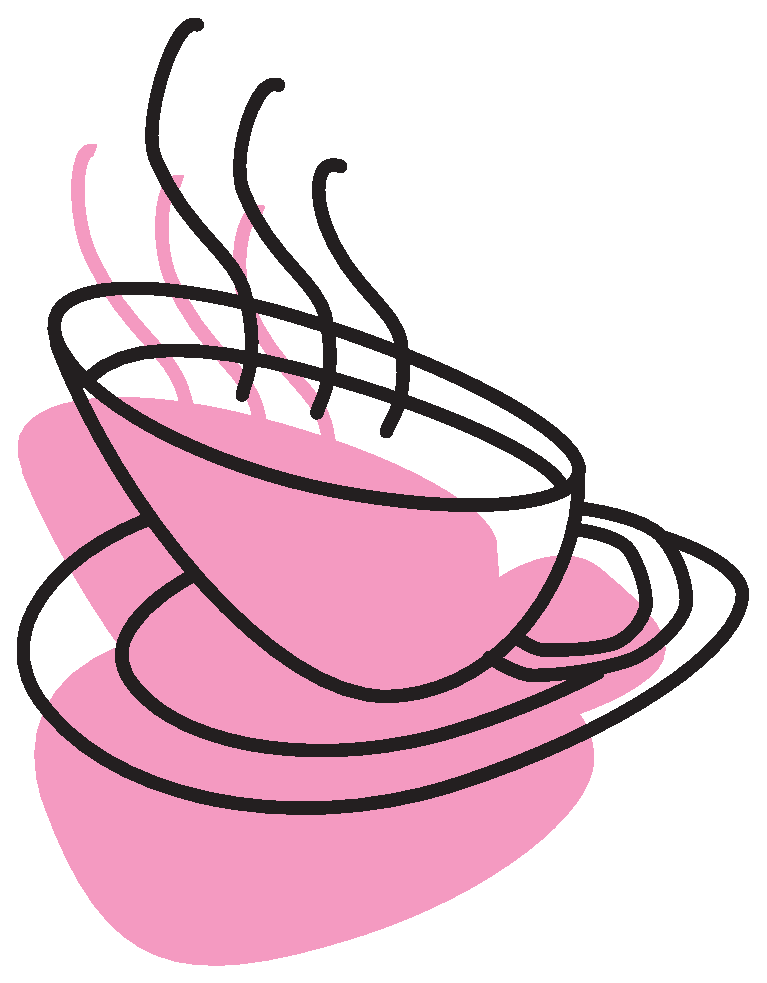
\includegraphics[width=6cm]{bilder/hyfs.eps}
\end{center}
\newpage

\inputsong{harjarevisan}
\inputsong{kalmarevisan}

\stepcounter{section}
\fancyfoot[RO,LE]{\large Punschvisor}
\begin{flushleft}
{\Huge Punschvisor\\}
\vspace{1cm}
\Large{
Punsch drickes antingen mycket kall till efterrätt alla dagar i veckan,
eller varm till torsdagens ärtsoppa. Det kan även hända att det
slinker ner en liten en till onsdags-hofflan. En gång i tiden hade
punschen systemets högsta apk - Alkohol per Krona - och många tror att
det är därför det alltid har druckits mycket punsch i studentikosa
sammanhang. Andra tror det beror på att det är gott.}
\end{flushleft}

\vspace{2cm}
\begin{center}
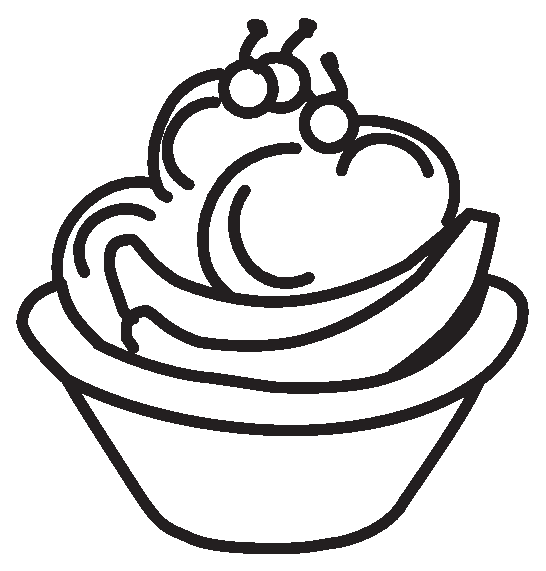
\includegraphics[width=5cm]{bilder/punsch.eps}
\end{center}
\newpage

\inputsong{gamlakall}
\inputsong{gamlavarm}
\newpage
\inputsong{punschvisaf}
\newpage
\inputsong{festu}
\inputsong{studiemedelsrondo}
\newpage
\inputsong{punschengul}
\inputsong{djungelpunsch}
\newpage
\inputsong{enkoppmedpunsch}
\newpage
\inputsong{gudarnaspunschvisa}
\inputsong{punschschottis}
\newpage
\inputsong{anglapunsch}
\newpage
\inputsong{punschlunch}
\inputsong{skogshogskolanspunschvisa}
\inputsong{jaggillar}
\newpage
\inputsong{arterochpunsch}
%\inputsong{narsompunschen}
\newpage
\inputsong{tvekaniforpunschen}
\newpage
\inputsong{punschpolkett}
\inputsong{minpunsch}
\newpage
\inputsong{punschpunsch}
\inputsong{punchpunch}
\newpage
\inputsong{vadjantillpunschen}
\inputsong{sistapunschvisan}

\stepcounter{section}
\fancyfoot[RO,LE]{\large Øhlvisor}
\begin{flushleft}
{\Huge Øhlvisor\\}
\end{flushleft}

\vspace{2cm}
\begin{center}

\includegraphics[width=6cm]{bilder/ohl.eps}
{\Large
\vspace{1cm}
Øhl är gott.
}
\end{center}
\newpage

\inputsong{odetillohlet}
\inputsong{lapinkulta}
\newpage
\inputsong{jagvarfullengang}
\newpage
\inputsong{minpilsner}
\inputsong{doremi}
\newpage
\inputsong{strejkpapripps}
\inputsong{knodejin}
\newpage
\inputsong{jumeraolvidricker}
\inputsong{pilsnerdrickaren}
\newpage
\inputsong{ohletsomforsvann}
%Byt ut
\inputsong{livetharsina}
\newpage
\inputsong{trivsel}
\inputsong{bottlesofbeer}
\inputsong{mellanolskvartett}

\stepcounter{section}
\stepcounter{section} % hoppa över F
\fancyfoot[RO,LE]{\large Vinvisor}
\begin{flushleft}
{\Huge Vinvisor\\}
\end{flushleft}

\vspace{2cm}
\begin{center}
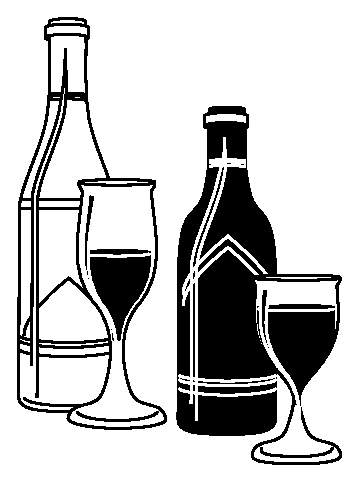
\includegraphics[width=6cm]{bilder/63.eps}

{\Large
\vspace{1cm}
In vino veritas}
\end{center}

\newpage
\begin{song}{Bordeaux, Bordeaux}{bordeaux}
\mel{I sommarens soliga dagar}
\begin{vers}
Jag minns än i dag hur min fader\\
kom hem i från staden så glader.\\
Han rada' upp flaskor i rader,\\
och sade nöjd som så: Bordeaux, Bordeaux!\\
Han drack ett glas, kom i extas,\\
och sedan blev det stort kalas.\\
Och vi små glin, ja vi drack vin,\\
som första klassens fyllesvin,\\
och vi dansade runt där på bordet\\
och skrek så vi blev blå:\\
Bordeaux, Bordeaux!\\
\end{vers}
\end{song}

\begin{song}{Nattvarden}{nattvarden}
\mel{We are all the winners}

\begin{vers}
Snabba på med vinet\\
söla inte präst\\
Strunta i oblaten, nu så är det fest\\
Skynda, fram med kalken\\
skit i orgelbrus och sång\\
Nu så ska vi ägna oss åt Nattvard dagen lång\\ 
\end{vers}
\end{song}

\newpage

\begin{song}{Vinet}{vinet}
\mel{Rullan går}
\begin{vers}
Vinet är ett märkligt ting,\\
märkligt ting, märkligt ting.\\
Bäst man känner ingenting,\\
ingenting, ingenting.\\
Vips man blir rätt yr i hatten,\\
dagen efter älskar vatten.\\
Men vad gör väl det ikväll?\\
Glaset höj, gutår och häll!\\
\end{vers}
\end{song}

\begin{song}{Sudda sudda}{suddasudda}
\begin{vers}
Sudda, sudda, sudda, sudda bort din sura min.\\
Med fyra jättestora bamseklunkar ädelt vin.\\
Munnen den skall sjunga och va' gla'.\\
För att den skall bli som den skall va'.\\
Vad häller du då bak det dolda flinet?\\
Vinet som suddar, suddar bort din sura min.\\
\end{vers}
\end{song}

\newpage

\begin{song}{Nu grönskar det}{nugronskardet}
\mel{Bondekantat}
\begin{vers}
Nu grönskar det i dalens famn, \\
nu doftar äng och lid.\\
Kom med, kom med på vandringsfärd\\
i vårens glada tid!\\
Var dag är som en gyllne skål,\\
till brädden fylld med vin.\\
så drick, min vän, drick sol och doft,\\
ty dagen den är din.\\
\end{vers}
\begin{vers}
Långt bort från stadens gråa hus \\
vi glatt vår kosa styr.\\
Och följer vägens vita band\\
mot ljusa äventyr.\\
Med öppna ögon låt oss se\\
på livets rikedom\\
som gror och sjuder överallt\\
där våren går i blom!\\
\end{vers}
\end{song}

\newpage

\begin{song}{Feta fransyskor}{fetafransyskor}
\mel{Marsche militaire}
\begin{vers}
Feta fransyskor som svettas om fötterna\\
de trampar druvor som sedan skall jäsas till vin\\
Transpirationen viktig e'\\
ty den ger fin bouquet\\
Vårtor och svampar följer me',\\
men vad gör väl de'?\\
\end{vers}
\begin{vers}
För...\\
\end{vers}
\begin{vers}
Vi vill ha vin, vill ha vin, vill ha mera vin\\
även om följderna bli att vi må lida pin\\
\textit{Flickor:}   Flaskan och glaset gått i sin.\\
\textit{Pojkar:}    Hit med vin, mera vin!\\
\textit{Flickor:}   Tror ni att vi är fyllesvin?\\
\end{vers}
\begin{vers}
JA! (Fast större)\\
\end{vers}
\end{song}

\newpage

\begin{song}{Undulaten}{undulaten}
\mel{Med en enkel tulpan}

\begin{vers}
Jag är en liten undulat\\
som får så dåligt med mat\\
för dom jag bor hos\\
ja dom jag bor hos\\
dom är så snåla.\\
Jag får ju fisk varenda dag\\
men det vill jag inte ha\\
jag vill ha rödvin\\
jag vill ha rödvin och gorgonzola\\
\end{vers}
\end{song}


\begin{song}{Ta ett glas}{taettglas}
\mel{Oh Tannenbaum}

\begin{vers}
Oh, ta ett glas,\\
Oh, ta ett glas.\\
Ty vinet för oss samman.\\
Och den som inget glas vill ha,\\
han sjunger och är lika gla'.\\
Men ta ett glas,\\
ja ta ett glas,\\
för livets fröjd och gamman.\\
\end{vers}
\end{song}

\newpage

\begin{song}{Vårvinets lov}{varvinetslov}
\mel{I sommarens soliga dagar}

\begin{vers}
Se, vinet det glimmar i glasen,\\
av vin blir det glatt på kalasen.\\
Sopranen, tenoren och basen\\
vid Bacchi hov\\
vill sjunga vinets lov.\\
Därför ej dröj - pokalen höj\\
och dig med druvans saft förnöj.\\
En nektar som vi tycker om\\
och återverkar småningom.\\
I vårdagars roliga stunder\\
ett glatt och fylligt vin är melodin!\\ 
\end{vers}
\end{song}

\begin{song}{Elysisk längtan}{elysisklangtan}
\mel{An die Freude}
\begin{vers}
Aftonrodnan svalka sprider\\
skymningen sig sänker fin\\
och likt dimridåer sprider\\
doften av det rena vin\\
\end{vers}
\begin{vers}
//: Låt det hjälpa mig till att segla\\
rakt in i rusets röda tröst\\
natten flyr på gryningsvingar\\
värmen flammar i mitt bröst ://\\
\end{vers} 
\end{song}

\newpage

\begin{song}{Så länge rösten är mild}{salangerosten}
\mel{Så länge skutan kan gå}
\begin{vers}
Så länge rösten är mild\\
så länge ingen är vild\\
så länge spegeln på väggen\\
ger halvskaplig bild\\
Så länge alla kan stå\\
så länge alla kan gå\\
så länge alla kan tralla så fyller vi på\\
\end{vers}
\begin{vers}
För vem har sagt att\\
just du kom med storken\\
för att bli glad\\
av att lukta på korken\\
Så till kvinns och till mans\\
vi höjer bägar'n med glans\\
och låter vinet gå ner\\
i en yrande dans\\
\end{vers}
\end{song}




\stepcounter{section}
\fancyfoot[RO,LE]{\large Bellman}
\begin{flushleft}
\section{Bellmanvisor}
{\Large Carl Michael Bellman (1740-1795) hör till de största svenska skalderna.
Han levde ett glatt liv i Stockholm och sågs ofta på societetskrogen Den Gyllene Freden, liksom på sjaskiga hak på Södermalm.
I dessa miljöer fann Bellman sin inspiration till visornas mustiga karaktärer - Movitz, Fredman, Ulla Winblad...
Vi gillar Bellman och har därför givit hans visor ett eget kapitel i Encyclopedia Gasquica.}
\end{flushleft}

\vspace{2cm}
\begin{center}
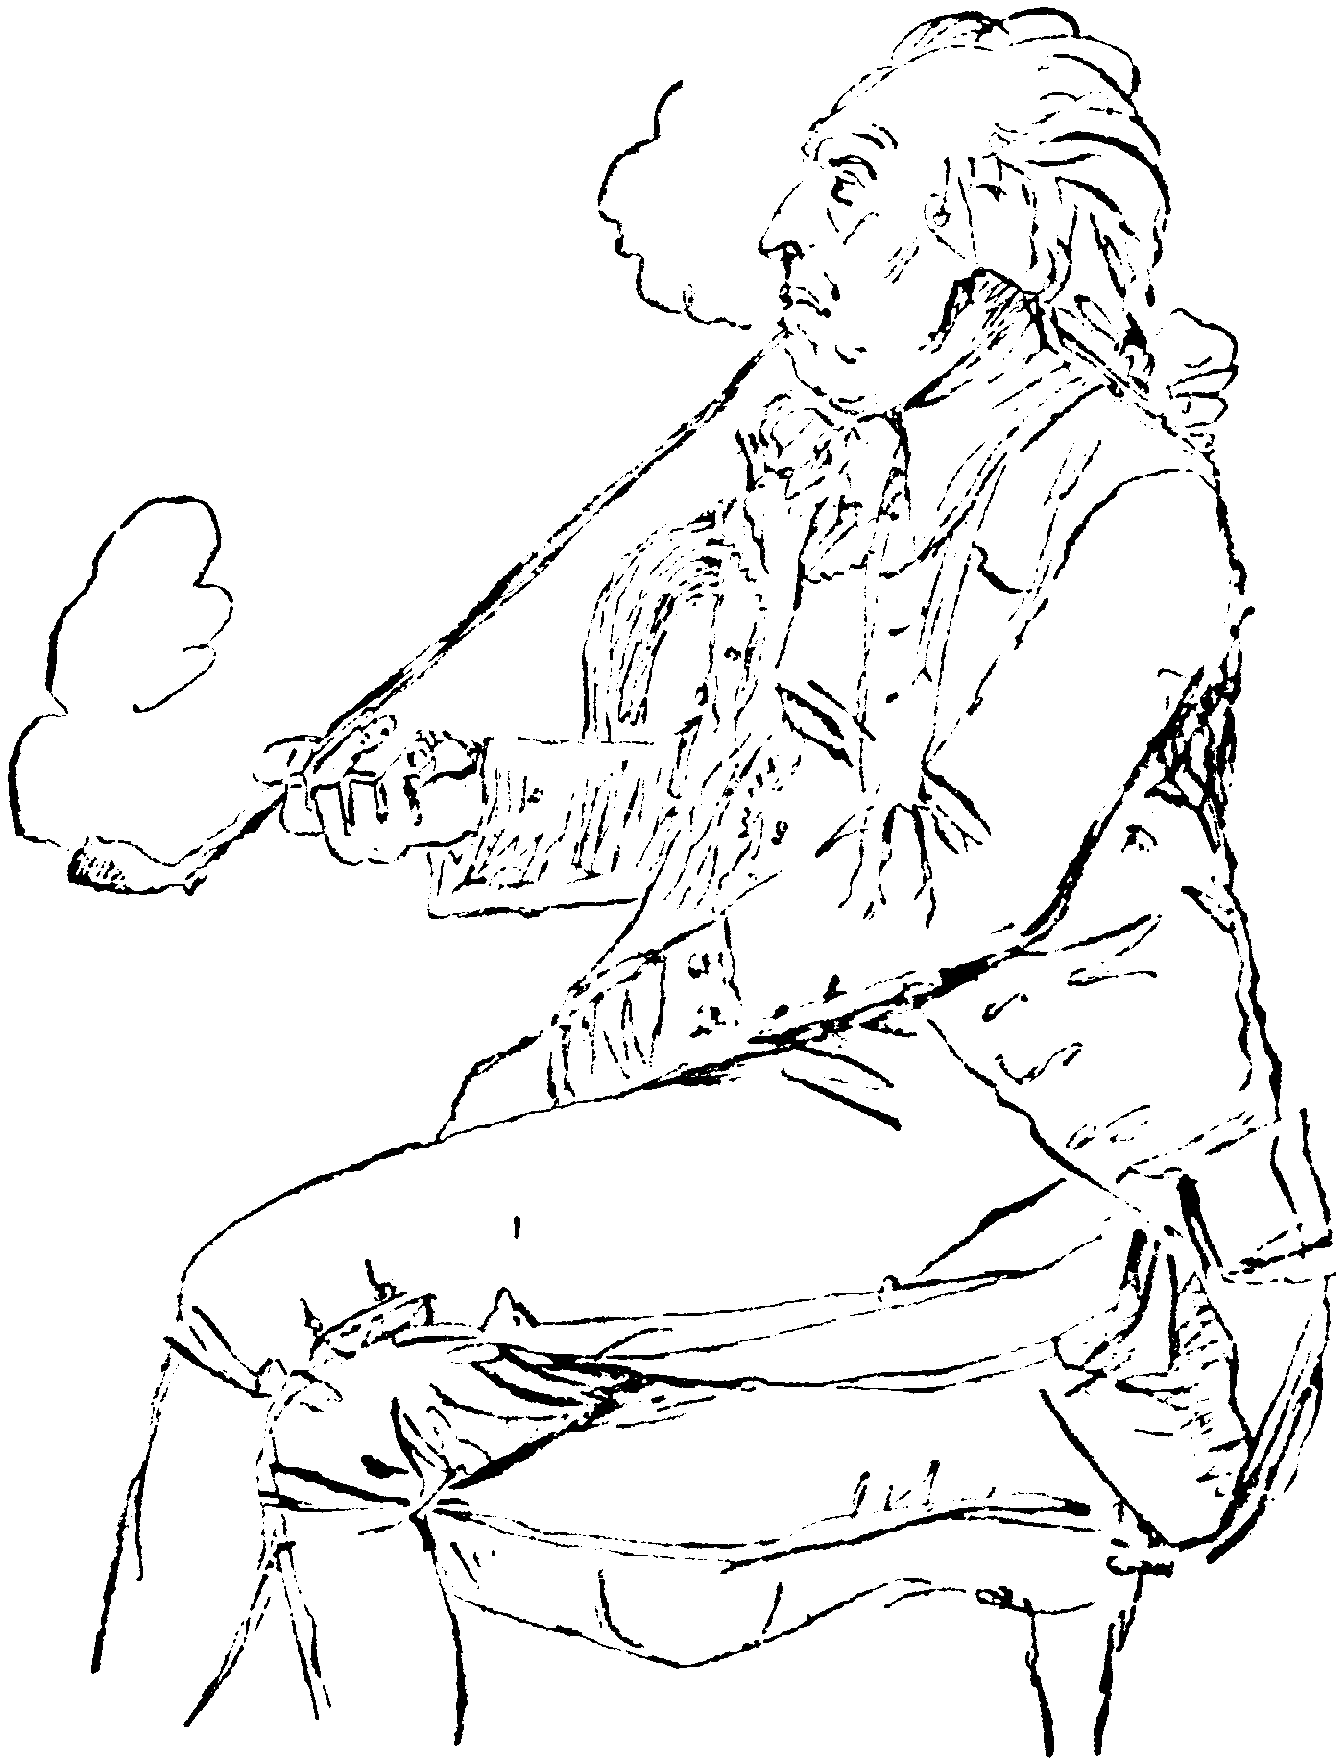
\includegraphics[width=6cm]{bilder/bellman.png}
\end{center}
\newpage

\inputsong{fredmanssangno35}
\inputsong{fjarilnvingad}
\inputsong{fredmanssangno21}
\newpage
\inputsong{epistel81}
\newpage
\inputsong{epistel01}
\newpage
\inputsong{solenglimmar}
\kom{(Då orginalsången har 21 verser valde\\
vi att ta med den första och sista)}
%Liksom en herdinna


\stepcounter{section}
\fancyfoot[RO,LE]{\large Övriga}
\begin{flushleft}
\section{Övriga sånger}
{\Large
Sångförmannen säger:
- Sjung! Sjung på sittningar, sjung på vardagar, sjung idag, sjung
imorgon, sjung för jämnan. Sjung hellre än bra! Här följer en mängd härliga sånger, vissa
med roliga texter, vissa som sjungs vid speciella tillfällen och vissa
som faktiskt är riktigt bra. Håll till godo!
}
\end{flushleft}

\vspace{2cm}
\begin{center}

\includegraphics[width=7cm]{bilder/sjung.eps}
\end{center}
\newpage

\inputsong{integralvisan}
\newpage
%Vers 2 och 3 tillagda av Jas, 2011
\inputsong{kaffesang}
\inputsong{barnermigtillsjon}
\newpage
\inputsong{treo}
%Tillagd av Jas, 2011
\inputsong{drickaalkohol}
\newpage
\inputsong{faderabraham}
\inputsong{fritiof}
\newpage
\inputsong{nikolajev}
\inputsong{stockholmsvisan}
\newpage
% Utbytt mot avtackningsången efter Dryckesregler
%\inputsong{detvarivarungdom}
\newpage
\inputsong{brevfrankolonien}
\newpage
\inputsong{drunkensailor}
\newpage
%Whiskeysången
%Återinförd av Jas, 2011
\inputsong{theballofkerrymuir}
%Tillagd av Jas, 2011
\inputsong{utiminmage}
\newpage
\inputsong{finskteknologvisa}
\newpage
%Tillagd av Jas, 2011
\inputsong{majdagen}
\inputsong{chalmeristvisa}
\inputsong{raven}
\newpage
\inputsong{pellejons}
\inputsong{toreador}
\newpage
\inputsong{anglamark}
\newpage
\inputsong{rovarnasvisa}
\newpage
\inputsong{balladkaxigamyran}
\inputsong{utivarhage}
\newpage
\inputsong{schottispavalhall}
\newpage
\inputsong{balladfredrik}
%Tillagd av Jas, 2011
\inputsong{dagenefter}
\inputsong{fritiofmarsch}
\newpage
\inputsong{enkungensman}
\newpage
\inputsong{balladbriggen}
%Grill 2014. Hämtad från cret. Alltså lundare i Val d'Isere.
\inputsong{finland}


\stepcounter{section}
\fancyfoot[RO,LE]{\large Julvisor}
\begin{flushleft}
{\Huge Julvisor\\}
{\Large
\vspace{1cm}
Julen infaller 24 december varje år och firas till minne av Kristi
födelse. Lucia infaller mitt i tentaveckan i läsperiod två och firas
till minne av Lucias död.}
\end{flushleft}
\vspace{2cm}
\begin{center}

\includegraphics[width=6cm]{bilder/112.eps}

\end{center}

\newpage

\begin{song}{Hej tomtegubbar}{hejtomtegubbar}
\begin{vers}
Hej tomtegubbar slå i glasen\\
och låt oss lustiga vara.\\
Hej tomtegubbar slå i glasen\\
och låt oss lustiga vara.\\
En liten tid vi leva här\\
med mycken möda och stort besvär.\\
Hej tomtegubbar slå i glasen\\
och låt oss lustiga vara.\\
\end{vers}
\end{song}

\begin{song}{Nu har vi ljus}{nuharviljus}
\begin{vers}
Nu har vi ljus här i vårt hus,\\
julen är kommen, hopp fa-ra-la-la!\\
Barnen i ring dansa omkring,\\
dansa omkring.\\
Granen står så grön och grann i stugan,\\
granen står så grön och grann i stugan.\\
Tra-la-la-la-la, tra-la-la-la-la,\\
ra-la-la-la-la, la-la!\\
\end{vers}
\end{song}
\newpage

\begin{song}{Nu är det jul igen}{nuardetjuligen}
\begin{vers}
//: Nu är det jul igen, och nu är det jul igen,\\
och julen varar än till påska. ://\\
//: Men det var inte sant, och det var inte sant,\\
för däremellan kommer fasta. ://\\
\end{vers}
\end{song}


\begin{song}{Rudolf med röda mulen}{rudolfmedrodamulen}
\begin{vers}
Rudolf med röda mulen\\
hette en helt vanlig ren\\
som blivit kall om mulen,\\
därav kom dess röda sken.\\
Rudolf fick alltid höra\\
"Se, han har sitt dimljus på",\\
att han blev led på detta,\\
det är sånt man kan förstå.\\
\end{vers}
\begin{vers}
Men en mörk julaftonskväll\\
Tomtefar han sa:\\
"Vill du inte Rudolf säg,\\
med din mule lysa mig."\\
Allt se'n den da'n den renen\\
tomtens egen släde drar.\\
Rudolf med röda mulen\\
lyser väg för tomtefar.\\
\end{vers}
\end{song}

\newpage

\begin{song}{Sankta Lucia}{sanktalucia}
\begin{vers}
Natten går tunga fjät runt gård och stuva.\\
Kring jord som sol förgät, skuggorna ruva.\\
Då i vårt mörka hus, stiger med tända ljus,\\
Sankta Lucia, Sankta Lucia.\\
\end{vers}
\begin{vers}
Natten var stor och stum. Nu hörs det svingar,\\
i alla tysta rum, sus som av vingar.\\
Se på vår tröskel står vitkläd, med ljus i hår,\\
Sankta Lucia, Sankta Lucia.\\
\end{vers}
\end{song}

\begin{song}{Glöggvisa}{gloggvisa}
\mel{Och jungfrun hon går i dansen med röda gullband}
\begin{vers}
Ack, glöggen den står på bordet och ångar sig varm\\
vi häller den ner i halsen och värmer vår tarm.\\
En här, en där, utan minsta besvär\\
den drycken är vår strupe så innerligt kär\\
\end{vers}
\end{song}

\begin{song}{Nu tändas tusen juleljus}{nutandas}
\begin{vers}
Nu tändas tusen juleljus på jordens mörka rund.\\
Och tusen, tusen strålar ock på himlens djupblå grund.\\
För över stad och land i kväll går julens glada bud.\\
Att född är herren Jesus Krist, vår frälsare och Gud.
\end{vers}
\end{song}

\begin{song}{Staffansvisan}{staffansvisan}
\begin{vers}
Staffan var en stalledräng,\\
vi tackom nu så gärna.\\
Han vattnade sina fålar fem,\\
allt för den ljusa stjärna.\\
Ingen dager synes än,\\
stjärnorna på himmelen de blänka.\\
\end{vers}
\begin{vers}
Två de voro röda, vi tackom nu så gärna.\\
de tjänte väl sin föda, allt för den ljusa stjärna.\\
Ingen dager...\\
\end{vers}
\begin{vers}
Två de voro vita, vi tackom nu så gärna.\\
de va varandra lika, allt för den ljusa stjärna.\\
Ingen dager...\\
\end{vers}
\begin{vers}
Den femte den var apelgrå, vi tackom nu så gärna.\\
den rider Staffan själv uppå, allt för den ljusa stjärna.\\
Ingen dager...\\
\end{vers}
\begin{vers}
Innan hanen galigt har, vi tackom nu så gärna.\\
Staffan uti stallet var, allt för den ljusa stjärna.\\
Ingen dager...\\
\end{vers}
\end{song}
\newpage

\begin{song}{Stilla natt}{sillanatt}
\begin{vers}
Stilla natt, heliga natt,\\
allt är frid, stjärnan blid\\
skiner på barnet i stallets strå,\\
och de vakande fromma två.\\
Kristus till jorden är kommen,\\
oss är en frälsare född.\\
\end{vers}
\begin{vers}
Stora stund, heliga stund,\\
änglars här går sin rund\\
kring de vaktande herdarnas hjord.\\
Rymden ljuder av glädjens ord:\\
Kristus till jorden är kommen,\\
eder är frälsaren född.\\
\end{vers}
\begin{vers}
Stilla natt, heliga natt,\\
mörkret flyr, dagen gryr.\\
Räddningstimmen för världen slår,\\
nu begynner vårt ljubelår.\\
Kristus till jorden är kommen,\\
oss är en frälsare född.\\
\end{vers}
\end{song}

\newpage

\begin{song}{Tomtarnas julnatt}{tomtarnasjulnatt}
\begin{vers}
Midnatt råder, tyst det är i husen, tyst i husen.\\
Alla sova, släckta äro ljusen, äro ljusen.\\
Tipp-tapp, tipp-tapp,\\
tippe-tippe-tipp-tapp.\\
Tipp, tipp, tapp.\\
\end{vers}
\begin{vers}
Se, då krypa tomtar upp ur vrårna, upp ur vrårna.\\
Lyssna, speja, trippa fram på tårna, fram på tårna.\\
Tipp-tapp...\\
\end{vers}
\begin{vers}
Snälla folket låtit maten rara, maten rara,\\
stå på bordet åt en tomteskara, tomteskara.\\
Tipp-tapp...\\
\end{vers}
\begin{vers}
Hur de mysa, hoppa upp bland faten, upp bland faten.\\
Tissla, tassla: "God är julematen, julematen.\\
Tipp-tapp...\\
\end{vers}
\begin{vers}
Se, då krypa tomtar upp ur vrårna, upp ur vrårna.\\
Lyssna, speja, trippa fram på tårna, fram på tårna.\\
Tipp-tapp...\\
\end{vers}
\begin{vers}
Snälla folket låtit maten rara, maten rara,\\
stå på bordet åt en tomteskara, tomteskara.\\
Tipp-tapp...\\
\end{vers}
\newp
\begin{vers}
Hur de mysa, hoppa upp bland faten, upp bland faten.\\
Tissla, tassla: "God är julematen, julematen".\\
Tipp-tapp...\\
\end{vers}
\begin{vers}
Gröt och skinka, lilla äppelbiten, äppelbiten.\\
Tänk så rart det smakar Nisse liten, Nisse liten.\\
Tipp-tapp...\\
\end{vers}
\begin{vers}
Nu till lekar, glada skrattet klingar, skrattet klingar.\\
Runt om granen skaran muntert svingar, muntert svingar.\\
Tipp-tapp...\\
\end{vers}
\begin{vers}
Natten lider. Snart de tomtar snälla, tomtar snälla,\\
kvickt och näpet allt i ordning ställa, i ordning ställa.\\
Tipp-tapp...\\
\end{vers}
\begin{vers}
Sedan åter in i tysta vrårna, tysta vrårna,\\
tomteskaran tassar nätt på tårna, nätt på tårna.\\
Tipp-tapp...\\
\end{vers}
\end{song}


\stepcounter{section}
\fancyfoot[RO,LE]{\large Djungelvrål}
\begin{flushleft}
{\Huge Djungelvrål\\}
{\Large
\vspace{1cm}
Ute i skogen är det mörkt, kallt och läskigt. Om man blir rädd eller
bara är lite orolig finns det inget bättre än att samstämt lätta på
rädslan i glad sång. Skuggorna bakom träden försvinner, humöret växer
och lägerelden värmer än bättre. Om ni är på hajk, på svamputflykten eller på
orienteringsrundan kan ni med fördel sjunga dessa sånger.}
   
\end{flushleft}
\vspace{2cm}
\begin{center}

\includegraphics[width=6cm]{bilder/120.eps}

\end{center}
 

\newpage
\begin{song}{ABC}{abc}
\begin{vers}
Timmen är slagen nu slutar vi för dagen,\\
går hem till mig, jag skall förhöra dig.\\
\end{vers}
\begin{vers}
ABC, du är i mina tankar\\
CDE, mitt hjärta det bankar,\\
EFG, du får mig alltför lätt ur balans.\\
ABC, du är i mina tankar\\
CDE, mitt hjärta det bankar,\\
EFG, du ger mig ingen ärlig chans.\\
\end{vers}
\begin{vers}
Du är den bästa i hela klassen, i biologi.\\
Du läser på till och med på rasten om kärlekens kemi.\\
Du är inte som alla andra.\\
Du är min första kärlek.\\
Du är alla tjejernas dröm.\\
Matematik, tillsammans är vi två.\\
Som ljuv musik, do re mi fa so la-a-a-a.\\
\end{vers}
\begin{vers}
ABC, du är i mina tankar\\
CDE, mitt hjärta det bankar,\\
EFG, du ger mig ingen ärlig chans.\\
\end{vers}
\begin{vers}
Jag känner nånting, ja det händer nånting,\\
det är nånting som brinner i mig.\\
Kärleken vaknar, å vad jag saknar,\\
känslan att hålla i dig.\\
Biologi, är kärlekens magi.\\
Min melodi, ikväll så är jag fri-i-i-i-i.\\
\end{vers}
\begin{vers}
ABC, du är i mina tankar\\
CDE, mitt hjärta det bankar,\\
EFG, du får mig alltför lätt ur balans.\\
ABC, du är i mina tankar\\
CDE, mitt hjärta det bankar,\\
EFG, du ger mig ingen ärlig chans.\\
ABC, du ger mig ingen ärlig chans.\\
\end{vers}
\end{song}

\begin{song}{The lion sleeps tonight}{thelion}
\begin{vers}
In the jungle, the mighty jungle, \\
the lion sleeps tonight.\\
In the jungle, the mighty jungle, \\
the lion sleeps tonight.\\
Wee-ooh wim-o-weh.\\
//: Wim-o-weh o-wim-o-weh o-wim-o-weh o-wim-o-weh\\
o-wim-o-weh o-wim-o-weh o-wim-weh. ://\\
\end{vers}
\begin{vers}
Near the village, the peaceful village, \\
the lion sleeps tonight.\\
Near the village, the peaceful village, \\
the lion sleeps tonight.\\
Wee-ooh wim-o-weh...\\
Hush, my darling, don't fear, my darling, \\
the lion sleeps tonight.\\
Hush, my darling, don't fear, my darling, \\
the lion sleeps tonight.\\
Wee-ooh wim-o-weh...\\
\end{vers}
\end{song}

\newpage

\begin{song}{Fantomens brallor}{fantomensbrallor}
\begin{vers}
Ingen har sett Fantomen utan kläder\\
klädd i pyjamas och stövlar av läder.\\
Han drar nog bort en rand där fram\\
när han kissar bakom trädets stam.\\
\end{vers}
\begin{vers}
Refr:\\
O, vandrande vålnad, kliar inte sviden\\
när du knegar i djungeln hela tiden?\\
Gör som Guran, skaffa dig en kjol,\\
det är bättre under Afrikas sol.\\
\end{vers}
\begin{vers}
Ingen har sett honom kavla upp ärmen\\
ljusblå lekdräkt i fukten och värmen.\\
Men han blev nog frusen om sin häck\\
Om han satt i grottan alldeles näck.\\
\end{vers}
\begin{vers}
Refr\\
\end{vers}
\begin{vers}
Fantomen lättar inte på kalsongen\\
nej, han håller värmen stången.\\
Ibland tar han på sig ännu mer\\
när Mr Walker sig till staden beger.\\
\end{vers}
\begin{vers}
Refr\\
\end{vers}
\end{song}

\newpage

\begin{song}{Kung Louis sång}{kingloui}
\begin{vers}
Jag kungen är över alla här\\
under trädens gröna höjd.\\
Jag har nått opp, till högsta topp,\\
men ännu är jag ej nöjd.\\
Jag vill ju va en man, en mänska, \\
och kunna allt Ni kan.\\
Jag vill inte längre apa mig, \\
jag vill ju bara va en man.\\
\end{vers}
\begin{vers}
Refr:\\
Oh, obido. Jag vill va som du.\\
Jag vill se ut som du, gå som du-u-u.\\
Det vill jag nu, ett djur som jag. (ubi dubi dubi)\\
Det lär sig bra bli en människa.\\
\end{vers}
\begin{vers}
Försök inte lura mig gosse, \\
jag inga konster tål.\\
Att känna till hur eld blir till, \\
det är mina drömmars mål.\\
Din hemlighet vill jag veta, \\
seså säg hur det går till.\\
För då blir jag visst, en man till sist, \\
och det är ju vad jag vill.\\
\end{vers}
\begin{vers}
Refr\\
\end{vers}
\end{song}

\begin{song}{Var nöjd med allt som livet ger}{varnojd}
\begin{vers}
Var nöjd med allt som livet ger \\
och allting som du kring dig ser,\\
glöm bort bekymmer, sorger och besvär. \\
Var glad och nöjd, för vet du vad? \\
En björntjänst gör ju ingen glad.\\
Var nöjd med livet som vi lever här. \\
Varthän jag än strövar, varthän jag än går \\
står ljung och snår kring mina spår. \\
Jag älskar bin och deras bon, \\
för honung är ju min passion\\
och vill du av myror ha munnen full \\
så ta en titt under sten och mull.\\
- Äta myror?\\
- Ha, ha, det är världens käk.\\
Kittlar dödsskönt i kistan. \\
Var nöjd med allt du ser och allt som livet ger.\\
Var nöjd...\\
Om frukter dig lockar, banan eller bär.\\
Se till att du plockar dem utan besvär. \\
Vill du plocka frukt av bästa klass \\
så använd din höger och vänster tass, \\
men klorna dom skall du dra in\\
så fort du ska ta dig en fin apelsin.\\
- Hoppas att du har förstått?\\
- O, ja! Tack Baloo!\\
Var nöjd...\\
\end{vers}
\end{song}


\begin{song}{Patrullmans sång}{patrullmanssang}
\mel{House of the Rising Sun}
\begin{vers}
Jag har ett glas uti min hand\\
till brädden fyllt med sprit.\\
Jag tar mig så en tår på tand,\\
en Skåne Akvavit.\\
\end{vers}
\begin{vers}
Patrullman, broder, om du vill,\\
drick ur tills du blir nöjd.\\
Skåla sedan alla till\\
i gamman och i fröjd.\\
\end{vers}
\end{song}

\newpage

\begin{song}{Ode till valen Åke}{valenake}
\mel{ABC}
\begin{vers}
Timmen är slagen,\\
nu strandar du på magen,\\
har gått iland,\\
i Träslövsläges hamn.\\
\end{vers}
\begin{vers}
ÅKE, nu har du strandat.\\
VAL, för alltid du landat.\\
DÖD, du kommer aldrig simma igen.\\
\end{vers}
\begin{vers}
Du var den bästa i hela havet,\\
på att fånga sill.\\
Nu är du fast i museets monter,\\
nu ligger du still.\\
Du är inte som alla andra Ååååke.\\
Du är vår hedersmedlem,\\
du är alla F-ares vän.\\
\end{vers}
\begin{vers}
ÅKE, nu har du strandat.\\
VAL, för alltid du landat.\\
DÖD, du kommer aldrig simma igen.\\
\end{vers}
\end{song}














\stepcounter{section}
\fancyfoot[RO,LE]{\large Register}
\begin{flushleft}
\section{Register}
\end{flushleft}
\begin{longtable}[h]{@{}p{\linewidth}@{}}% en kolumn som fyller hela sidan
\endfirsthead
\endhead
\endfoot
\endlastfoot  \hyperref[etttva]{1 2 75 6 7}\dotfill\hyperref[etttva]{B.40}\\
  \hyperref[tjutrean]{23:an}\dotfill\hyperref[tjutrean]{B.18}\\
  \hyperref[bottlesofbeer]{99 bottles of beer on the wall}\dotfill\hyperref[bottlesofbeer]{E.9}\\
  \hyperref[varmeland]{Ack Värmeland du sköna}\dotfill\hyperref[varmeland]{A.6}\\
  \hyperref[alkemisten]{Alkemisten}\dotfill\hyperref[alkemisten]{B.13}\\
  \hyperref[alkonalen]{Alkonålen}\dotfill\hyperref[alkonalen]{B.50}\\
  \hyperref[avundsjukvisa]{Avundsjuk visa}\dotfill\hyperref[avundsjukvisa]{B.33}\\
  \hyperref[bordeaux]{Bordeaux, Bordeaux}\dotfill\hyperref[bordeaux]{G.1}\\
  \hyperref[bordsvisa]{Bordsvisa}\dotfill\hyperref[bordsvisa]{B.42}\\
  \hyperref[brevfrankolonien]{Brev från kolonien}\dotfill\hyperref[brevfrankolonien]{I.8}\\
  \hyperref[byssanlull]{Byssan lull}\dotfill\hyperref[byssanlull]{B.20}\\
  \hyperref[chalmeristvisa]{Chalmeristvisa}\dotfill\hyperref[chalmeristvisa]{I.10}\\
  \hyperref[dvisorsvenska]{D-visor (Svenska)}\dotfill\hyperref[dvisorsvenska]{B.47}\\
  \hyperref[yndigtland]{Det er et yndigt land}\dotfill\hyperref[yndigtland]{A.4}\\
  \hyperref[djungelpunsch]{Djungelpunsch}\dotfill\hyperref[djungelpunsch]{D.7}\\
  \hyperref[doremi]{Do-Re-Mi-Beer}\dotfill\hyperref[doremi]{E.3}\\
  \hyperref[nyktra]{Dom som är nyktra}\dotfill\hyperref[nyktra]{B.32}\\
  \hyperref[dragosdragos]{Dragos, Dragos}\dotfill\hyperref[dragosdragos]{F.}\\
  \hyperref[dricksupentill]{Drick supen till}\dotfill\hyperref[dricksupentill]{B.49}\\
  \hyperref[drickaalkohol]{Dricka alkohol}\dotfill\hyperref[drickaalkohol]{I.2}\\
  \hyperref[dugamla]{Du gamla du fria}\dotfill\hyperref[dugamla]{A.1}\\
  \hyperref[elysisklangtan]{Elysisk längtan}\dotfill\hyperref[elysisklangtan]{G.10}\\
  \hyperref[bidragstagare]{En bidragstagare}\dotfill\hyperref[bidragstagare]{B.30}\\
  \hyperref[engangimanan]{En gång i månan}\dotfill\hyperref[engangimanan]{B.31}\\
  \hyperref[enkoppmedpunsch]{En kopp med punsch}\dotfill\hyperref[enkoppmedpunsch]{D.8}\\
  \hyperref[fyllhund]{En liten fyllhund}\dotfill\hyperref[fyllhund]{B.38}\\
  \hyperref[enters]{En ters}\dotfill\hyperref[enters]{B.28}\\
  \hyperref[entarpatanden]{En tår på tanden}\dotfill\hyperref[entarpatanden]{B.53}\\
  \hyperref[farensmorgon]{F-arens morgon}\dotfill\hyperref[farensmorgon]{B.43}\\
  \hyperref[faderabraham]{Fader Abraham}\dotfill\hyperref[faderabraham]{I.4}\\
  \hyperref[fantomensbrallor]{Fantomens brallor}\dotfill\hyperref[fantomensbrallor]{K.3}\\
  \hyperref[festu]{Festu:s punschvisa}\dotfill\hyperref[festu]{D.4}\\
  \hyperref[fetafransyskor]{Feta fransyskor}\dotfill\hyperref[fetafransyskor]{G.6}\\
  \hyperref[finland]{Finland}\dotfill\hyperref[finland]{I.16}\\
  \hyperref[finsksup]{Finsk supvisa}\dotfill\hyperref[finsksup]{B.55}\\
  \hyperref[fjarilnvingad]{Fjäriln vingad}\dotfill\hyperref[fjarilnvingad]{H.1}\\
  \hyperref[fritiof]{Fritiof och Carmencita - kort}\dotfill\hyperref[fritiof]{I.5}\\
  \hyperref[fullida]{Full ida'}\dotfill\hyperref[fullida]{B.34}\\
  \hyperref[gaffelnpafocus]{Gaffeln på Focus}\dotfill\hyperref[gaffelnpafocus]{I.18}\\
  \hyperref[gamlakall]{Gamla punschvisan (kall)}\dotfill\hyperref[gamlakall]{D.1}\\
  \hyperref[gamlavarm]{Gamla punschvisan (varm)}\dotfill\hyperref[gamlavarm]{D.2}\\
  \hyperref[gladjetaren]{Glädjetåren}\dotfill\hyperref[gladjetaren]{B.25}\\
  \hyperref[gloggvisa]{Glöggvisa}\dotfill\hyperref[gloggvisa]{J.6}\\
  \hyperref[fredmanssangno35]{Gubben Noak}\dotfill\hyperref[fredmanssangno35]{H.3}\\
  \hyperref[gudarnaspunschvisa]{Gudarnas punschvisa}\dotfill\hyperref[gudarnaspunschvisa]{D.9}\\
  \hyperref[halvan]{Halvan}\dotfill\hyperref[halvan]{B.5}\\
  \hyperref[hejtomtegubbar]{Hej tomtegubbar}\dotfill\hyperref[hejtomtegubbar]{J.1}\\
  \hyperref[helan]{Helan går}\dotfill\hyperref[helan]{B.1}\\
  \hyperref[hellandgore]{Hell and gore}\dotfill\hyperref[hellandgore]{B.2}\\
  \hyperref[harjarevisan]{Härjarevisan}\dotfill\hyperref[harjarevisan]{C.2}\\
  \hyperref[imbelupet]{Imbelupet}\dotfill\hyperref[imbelupet]{B.52}\\
  \hyperref[integralvisan]{Integralvisan}\dotfill\hyperref[integralvisan]{I.1}\\
  \hyperref[inversaptit]{Invers aptit}\dotfill\hyperref[inversaptit]{B.23}\\
  \hyperref[jamadendrickas]{Ja, må den drickas}\dotfill\hyperref[jamadendrickas]{B.4}\\
  \hyperref[vielsker]{Ja, vi elsker}\dotfill\hyperref[vielsker]{A.2}\\
  \hyperref[raven]{Jag fångade en räv en dag}\dotfill\hyperref[raven]{I.14}\\
  \hyperref[snusen]{Jag har aldrig var't på snusen}\dotfill\hyperref[snusen]{B.15}\\
  \hyperref[jagskallfesta]{Jag skall festa}\dotfill\hyperref[jagskallfesta]{B.39}\\
  \hyperref[jagvarfullengang]{Jag var full en gång}\dotfill\hyperref[jagvarfullengang]{E.1}\\
  \hyperref[jumeraolvidricker]{Ju mera öl vi dricker}\dotfill\hyperref[jumeraolvidricker]{E.7}\\
  \hyperref[kaisersmidsommarvisa]{Kaisers Midsommarvisa}\dotfill\hyperref[kaisersmidsommarvisa]{B.45}\\
  \hyperref[kalmarevisan]{Kalmarevisan}\dotfill\hyperref[kalmarevisan]{C.1}\\
  \hyperref[knodejin]{Knô dej in}\dotfill\hyperref[knodejin]{E.6}\\
  \hyperref[kingloui]{Kung Louis sång}\dotfill\hyperref[kingloui]{K.4}\\
  \hyperref[kungssangen]{Kungssången}\dotfill\hyperref[kungssangen]{A.5}\\
  \hyperref[karastebroder]{Käraste bröder}\dotfill\hyperref[karastebroder]{H.5}\\
  \hyperref[lapinkulta]{Lapin Kulta}\dotfill\hyperref[lapinkulta]{E.5}\\
  \hyperref[livet]{Livet}\dotfill\hyperref[livet]{A.7}\\
  \hyperref[lovsangtillsnapsen]{Lovsång till snapsen}\dotfill\hyperref[lovsangtillsnapsen]{B.51}\\
  \hyperref[lyftet]{Lyftet}\dotfill\hyperref[lyftet]{B.16}\\
  \hyperref[matlab]{Man ska ha MATLAB}\dotfill\hyperref[matlab]{I.13}\\
  \hyperref[mellanolskvartett]{Mellanölskvartett}\dotfill\hyperref[mellanolskvartett]{E.12}\\
  \hyperref[merabrannvin]{Mera brännvin}\dotfill\hyperref[merabrannvin]{B.6}\\
  \hyperref[mesen]{Mesen}\dotfill\hyperref[mesen]{B.10}\\
  \hyperref[minpilsner]{Min pilsner}\dotfill\hyperref[minpilsner]{E.2}\\
  \hyperref[minpunsch]{Min punsch}\dotfill\hyperref[minpunsch]{D.16}\\
  \hyperref[minnet]{Minnet}\dotfill\hyperref[minnet]{B.41}\\
  \hyperref[mittlillalan]{Mitt lilla lån}\dotfill\hyperref[mittlillalan]{B.35}\\
  \hyperref[moosen]{Moosen}\dotfill\hyperref[moosen]{B.9}\\
  \hyperref[musen]{Musen}\dotfill\hyperref[musen]{B.11}\\
  \hyperref[manen]{Månen}\dotfill\hyperref[manen]{B.8}\\
  \hyperref[masen]{Måsen}\dotfill\hyperref[masen]{B.7}\\
  \hyperref[nattvarden]{Nattvarden}\dotfill\hyperref[nattvarden]{G.2}\\
  \hyperref[nikolajev]{Nikolajev}\dotfill\hyperref[nikolajev]{I.6}\\
  \hyperref[nugronskardet]{Nu grönskar det}\dotfill\hyperref[nugronskardet]{G.5}\\
  \hyperref[nuharviljus]{Nu har vi ljus}\dotfill\hyperref[nuharviljus]{J.2}\\
  \hyperref[nutarviden]{Nu tar vi den}\dotfill\hyperref[nutarviden]{B.17}\\
  \hyperref[nutandas]{Nu tändas tusen juleljus}\dotfill\hyperref[nutandas]{J.7}\\
  \hyperref[nuardetjuligen]{Nu är det jul igen}\dotfill\hyperref[nuardetjuligen]{J.3}\\
  \hyperref[nubbenwalk]{Nubben walk}\dotfill\hyperref[nubbenwalk]{B.29}\\
  \hyperref[narsompunschen]{När som punschen}\dotfill\hyperref[narsompunschen]{D.20}\\
  \hyperref[naskruvafiolen]{Nå, skruva fiolen}\dotfill\hyperref[naskruvafiolen]{H.4}\\
  \hyperref[ohemskalabb]{O hemska labb}\dotfill\hyperref[ohemskalabb]{I.17}\\
  \hyperref[opriver]{O.P. river}\dotfill\hyperref[opriver]{B.19}\\
  \hyperref[oasen]{Oasen}\dotfill\hyperref[oasen]{B.37}\\
  \hyperref[valenake]{Ode till valen Åke}\dotfill\hyperref[valenake]{K.6}\\
  \hyperref[patrullmanssang]{Patrullmans sång}\dotfill\hyperref[patrullmanssang]{K.2}\\
  \hyperref[pilsnerdrickaren]{Pilsnerdrickaren}\dotfill\hyperref[pilsnerdrickaren]{E.11}\\
  \hyperref[porthos]{Porthos visa}\dotfill\hyperref[porthos]{B.14}\\
  \hyperref[punchpunch]{Punch, punch}\dotfill\hyperref[punchpunch]{D.18}\\
  \hyperref[punschpunsch]{Punsch, punsch}\dotfill\hyperref[punschpunsch]{D.17}\\
  \hyperref[punschlunch]{Punsch-lunch}\dotfill\hyperref[punschlunch]{D.12}\\
  \hyperref[punschengul]{Punschen gul}\dotfill\hyperref[punschengul]{D.6}\\
  \hyperref[punschpolkett]{Punschpolkett}\dotfill\hyperref[punschpolkett]{D.15}\\
  \hyperref[punschschottis]{Punschschottis}\dotfill\hyperref[punschschottis]{D.10}\\
  \hyperref[punschvisaf]{Punschvisa F}\dotfill\hyperref[punschvisaf]{D.3}\\
  \hyperref[rektorssangen]{Rektorssången}\dotfill\hyperref[rektorssangen]{A.9}\\
  \hyperref[rudolfmedrodamulen]{Rudolf med röda mulen}\dotfill\hyperref[rudolfmedrodamulen]{J.4}\\
  \hyperref[sanktalucia]{Sankta Lucia}\dotfill\hyperref[sanktalucia]{J.5}\\
  \hyperref[schottispavalhall]{Schottis på Valhall}\dotfill\hyperref[schottispavalhall]{I.15}\\
  \hyperref[sistapunschvisan]{Sista punschvisan}\dotfill\hyperref[sistapunschvisan]{D.21}\\
  \hyperref[solen]{Solen}\dotfill\hyperref[solen]{B.21}\\
  \hyperref[solenglimmar]{Solen glimmar blank och trind}\dotfill\hyperref[solenglimmar]{H.6}\\
  \hyperref[spritbolaget]{Spritbolaget}\dotfill\hyperref[spritbolaget]{B.36}\\
  \hyperref[staffansvisan]{Staffansvisan}\dotfill\hyperref[staffansvisan]{J.8}\\
  \hyperref[sillanatt]{Stilla natt}\dotfill\hyperref[sillanatt]{J.9}\\
  \hyperref[stockholmsvisan]{Stockholmsvisan}\dotfill\hyperref[stockholmsvisan]{I.7}\\
  \hyperref[strejkpapripps]{Strejk på Pripps}\dotfill\hyperref[strejkpapripps]{E.4}\\
  \hyperref[studentsangen]{Studentsången}\dotfill\hyperref[studentsangen]{A.8}\\
  \hyperref[studiebidrag]{Studiebidraget}\dotfill\hyperref[studiebidrag]{B.12}\\
  \hyperref[studiemedelsrondo]{Studiemedelsrondo}\dotfill\hyperref[studiemedelsrondo]{D.5}\\
  \hyperref[suddasudda]{Sudda sudda}\dotfill\hyperref[suddasudda]{G.4}\\
  \hyperref[systemeinternationale]{Systeme Internationale}\dotfill\hyperref[systemeinternationale]{B.46}\\
  \hyperref[fredmanssangno21]{Så lunka vi}\dotfill\hyperref[fredmanssangno21]{H.2}\\
  \hyperref[salangerosten]{Så länge rösten är mild}\dotfill\hyperref[salangerosten]{G.11}\\
  \hyperref[taettglas]{Ta ett glas}\dotfill\hyperref[taettglas]{G.8}\\
  \hyperref[thelion]{The lion sleeps tonight}\dotfill\hyperref[thelion]{K.1}\\
  \hyperref[thtyrkethaft]{Thtyrkethaft}\dotfill\hyperref[thtyrkethaft]{B.3}\\
  \hyperref[tomtarnasjulnatt]{Tomtarnas julnatt}\dotfill\hyperref[tomtarnasjulnatt]{J.10}\\
  \hyperref[toreador]{Toreador}\dotfill\hyperref[toreador]{I.9}\\
  \hyperref[treo]{Treo}\dotfill\hyperref[treo]{I.3}\\
  \hyperref[trivsel]{Trivsel}\dotfill\hyperref[trivsel]{E.8}\\
  \hyperref[tvekaniforpunschen]{Tvekan inför punschen}\dotfill\hyperref[tvekaniforpunschen]{D.14}\\
  \hyperref[omjaghade]{Tänk om jag hade}\dotfill\hyperref[omjaghade]{B.26}\\
  \hyperref[torstenrasar]{Törsten rasar}\dotfill\hyperref[torstenrasar]{B.48}\\
  \hyperref[undulaten]{Undulaten}\dotfill\hyperref[undulaten]{G.7}\\
  \hyperref[uppgasquening]{Uppgasquening}\dotfill\hyperref[uppgasquening]{B.54}\\
  \hyperref[utiminmage]{Uti min mage}\dotfill\hyperref[utiminmage]{I.12}\\
  \hyperref[varnojd]{Var nöjd med allt som livet ger}\dotfill\hyperref[varnojd]{K.5}\\
  \hyperref[vemkanragla]{Vem kan ragla}\dotfill\hyperref[vemkanragla]{B.44}\\
  \hyperref[vikingen]{Vikingen}\dotfill\hyperref[vikingen]{B.24}\\
  \hyperref[vilaviddennakalla]{Vila vid denna källa}\dotfill\hyperref[vilaviddennakalla]{H.7}\\
  \hyperref[vinet]{Vinet}\dotfill\hyperref[vinet]{G.3}\\
  \hyperref[vodkavodka]{Vodka vodka}\dotfill\hyperref[vodkavodka]{B.27}\\
  \hyperref[vadjantillpunschen]{Vädjan till punschen}\dotfill\hyperref[vadjantillpunschen]{D.19}\\
  \hyperref[vartland]{Vårt land}\dotfill\hyperref[vartland]{A.3}\\
  \hyperref[varvinetslov]{Vårvinets lov}\dotfill\hyperref[varvinetslov]{G.9}\\
  \hyperref[drunkensailor]{What shall we do with the drunken sailor}\dotfill\hyperref[drunkensailor]{I.11}\\
  \hyperref[anengang]{Än en gång däran}\dotfill\hyperref[anengang]{B.22}\\
  \hyperref[anglapunsch]{Änglapunsch}\dotfill\hyperref[anglapunsch]{D.11}\\
  \hyperref[arterochpunsch]{Ärter och punsch}\dotfill\hyperref[arterochpunsch]{D.13}\\
  \hyperref[angestvisan]{Ångestvisan}\dotfill\hyperref[angestvisan]{B.56}\\
  \hyperref[ohletsomforsvann]{Ölet som försvann}\dotfill\hyperref[ohletsomforsvann]{E.10}\\
\end{longtable}

\stepcounter{section}
\fancyfoot[RO,LE]{\large Sångförmän}
\begin{flushleft}
\section{Sångförmän}
\vspace{-1em}
\end{flushleft}

{\large
\setlength{\parskip}{0.5em}
\setlength\columnsep{3em}

\begin{multicols}{2}
\textbf{2019}\\
Alexandru Golic\\
David Hambraeus

\textbf{2018}\\
Felix Augustsson\\
Johanna ''Wärner'' Warnqvist\\
Alexandru Golic\\
David Hambraeus

\textbf{2017}\\
Johan ''Wello'' Winther\\
Gustaf ''Ampi'' Ström\\
Fredrik ''Ærnst'' Hallhagen\\
Felix Augustsson

\textbf{2016}\\
Johan ''Wello'' Winther\\
Gustaf ''Ampi'' Ström\\
Anders Fredriksson\\
Samuel Vrede\\
Fredrik ''Ærnst'' Hallhagen\\
Oskar Peetre

\textbf{2015}\\
Gustaf ''Ampi'' Ström\\
Lina ''Hallon'' Olandersson

\textbf{2014}\\
Navid ''Målsman'' Haddad\\
Holger ''JudÅ'' Lindström\\
Armin ''Grill'' Azhirnian

\textbf{2013}\\
Gustav Lindwall\\
Oskar ''KubN'' Fridell\\
Fredrik ''Flygplan'' Andersson

\textbf{2012}\\
Oskar ''KubN'' Fridell

\textbf{2011}\\
Amanda Gårdmark\\
Britta Thörnblom\\
Gustav Hansson

\textbf{2010}\\
Cecilia Kjellman

\textbf{2009}\\
Tomas Lovén

\textbf{2008}\\
Jonas Preisz\\
Daniel Gustafsson\\
Jonas Lindgren\\
Tomas Lovén

\textbf{Tidigare}\\
Dennis\\
Elmer\\
Kvickan

\end{multicols}
}


\end{document}
